% Auriga theme
% https://github.com/anishathalye/auriga

\documentclass[14pt,aspectratio=169]{beamer}
\usepackage{pgfpages}
\usepackage{fancyvrb}
\usepackage{booktabs,dcolumn}
\usepackage{tikz}
\usetikzlibrary{arrows.meta, positioning, quotes}
\usepackage{pgfplots}

% \ifnotes
% \setbeamertemplate{note page}[plain]
% \setbeameroption{show notes on second screen=right}
% \fi

\usetheme{auriga}
\usecolortheme{auriga}

% define some colors for a consistent theme across slides
\definecolor{red}{RGB}{181, 23, 0}
\definecolor{blue}{RGB}{0, 118, 186}
\definecolor{gray}{RGB}{146, 146, 146}

\title{Historia Económica Argentina}

\author{\underline{Sebastián Freille} \inst{1}}

\institute[shortinst]{\inst{1} IEF-UNC \\ UCC}
\date{}

\AtBeginSection[]{
    \begin{frame}
    \vfill
    \centering
    \begin{beamercolorbox}[sep=8pt,center,shadow=true,rounded=true]{title}
        \usebeamerfont{title}\insertsectionhead\par%
    \end{beamercolorbox}
    \vfill
    \end{frame}
}



\AtBeginSubsection[]{
    \begin{frame}
    \vfill
    \centering
    \begin{beamercolorbox}[sep=6pt,center,shadow=true,rounded=true]{title}
        \usebeamerfont{title}\insertsubsectionhead\par%
    \end{beamercolorbox}
    \vfill
    \end{frame}
}


\AtBeginSubsubsection[]{
    \begin{frame}
    \vfill
    \centering
    \begin{beamercolorbox}[sep=4pt,center,shadow=true,rounded=true]{title}
        \usebeamerfont{title}\insertsubsubsectionhead\par%
    \end{beamercolorbox}
    \vfill
    \end{frame}
}


\begin{document}

{
  % rather than use the frame options [noframenumbering,plain], we make the
  % color match, so that the indicated page numbers match PDF page numbers
  \setbeamercolor{page number in head/foot}{fg=background canvas.bg}
  \begin{frame}
    \titlepage
  \end{frame}
}

  
  \section{Capítulo 3. La Economía Política del Peronismo, 1946-1955}


  \section{Principales políticas y medidas}
  

 \begin{frame}\frametitle{Mayor rol del Estado}
    \begin{itemize}\itemsep 10pt
      \item Movimiento de un Estado no productor a un Estado productor
        \item Algunos hitos: 1) Estatización y nacionalización de los
          FFCC, 2) Horno siderúrgico (Zapala), 3) Nacionalización de
          teléfonos, 4) Creación de Yacimientos Carboníferos Fiscales
          (YCF), 5) Gas del Estado
          \item Estatizaciones fueron dirigidas principalmente a
            servicios públicos --no a frigoríficos y cementeras
            \item El principal partido opositor criticó las políticas
              de nacionalizaciones...por insuficiente!
                 \end{itemize}
               \end{frame}

               
               \begin{frame}\frametitle{Mayor rol del Estado (cont.)}
    \begin{itemize}\itemsep 10pt
      \item No alejado de lo que pasaba en la post-crisis y postguerra
        en países europeas con el Estado haciendose cargo de muchas
        actividades [clima de la epoca, ideas teóricas]
        \item Tendencia también ocurrida en América Latina
          --principales sectores generación electrica, construcción y
          transporte
          \item Ideas keynesiandas de tonificar DA y mantener altos
            niveles de empleo difundidas en muchos países
            \item Pero no sólo inversión pública $\longrightarrow$
              crece mucho el Estado de bienestar [seguridad social,
              seguros desempleo]
                 \end{itemize}
      \end{frame}



  \begin{frame}\frametitle{Mayor rol del Estado (cont.)}
\begin{figure}[hxtbp]\vspace{0cm}
  \centering
  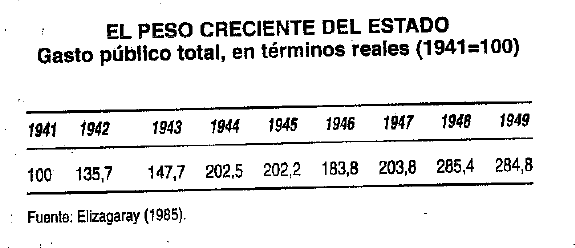
\includegraphics[scale=0.75]{uni3_politicas01}
   \label{fig:uni1_01}
\end{figure} 
  \end{frame}



   \begin{frame}\frametitle{Política de ingresos}
    \begin{itemize}\itemsep 10pt
    \item Primer Plan Quinquenal (Miranda) ven un fenomenal
      crecimiento del salario real (62\% de 1945 a 1949) --bastante
      por encima de crecimiento de productividad
      \item En 1948 distribución del PBI $\longrightarrow$ mas del
        53\% para el trabajo, resto para ganancias, intereses y rentas
        \item Idea de que aumentos salariales además de mayor
          bienestar directo causaban mayor DA por vía indirecta
          \item Fenomenal aumento del bienestar y consumo de la clase trabajadora
                 \end{itemize}
      \end{frame}




  \begin{frame}\frametitle{Política de ingresos (cont.)}
\begin{figure}[hxtbp]\vspace{0cm}
  \centering
  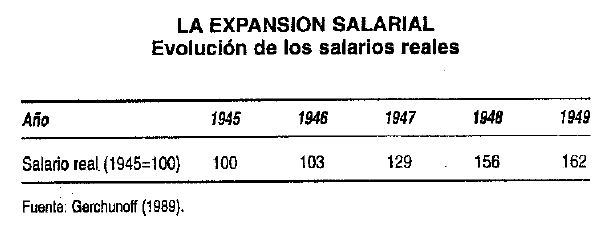
\includegraphics[scale=0.75]{uni3_politicas02}
   \label{fig:uni1_01}
\end{figure} 
  \end{frame}


      
   \begin{frame}\frametitle{Política de ingresos (cont.)}
    \begin{itemize}\itemsep 10pt
    \item Esta política de ingresos ocultaba una clara intencionalidad
      política de Perón --gana elecciones constituyentes de 1949 con
      66\% de los votos
    \item También se congelaron alquileres y algunos precios
    \item Política salarial basada en dos ejes.
      \begin{itemize}\itemsep 10pt \medskip
      \item garantizar pleno empleo
      \item redistribuir ingreso hacia sectores populares
      \end{itemize}
      \item También hubo redistribución via impuestos (aunque menor)
        $\longrightarrow$ mejoró progresividad de impuesto a la renta,
        creó impuestos al exceso de beneficios
                 \end{itemize}
      \end{frame}


\begin{frame}\frametitle{Política de ingresos (cont.)}
    \begin{itemize}\itemsep 10pt
    \item Pero sin duda la parte del león de los ingresos fiscales
      vinieron dados por el sistema de seguridad social
      $\longrightarrow$ creado en 1904, el sistema se expandió varias
      veces hasta que entre 1944-46 se crearon las cajas para
      empleados de comercio y de obreros industriales
      \item Sistema de cajas era ampliamente superavitario (recursos
        un 4\% del
        PBI)  --no había
        beneficiarios
        \item  La redistribución, por tanto, tuvo lugar
          mayoritariamente a través de política salarial y no de
          gastos/impuestos. ¿De donde salieron esos fondos?
                 \end{itemize}
      \end{frame}



      
\begin{frame}\frametitle{Desarrollo industrial}
    \begin{itemize}\itemsep 10pt
    \item Impulso a la industrialización sustitutiva de importaciones promovida desde el Estado
      basado en varias razones:
      \begin{itemize}\itemsep 10pt \medskip
      \item Nacionalismo
      \item Mantenimiento de empleo y consumo alto
      \item Eje de desarrollo a largo plazo
        \item Sentimiento e ideas desarrollistas de organismos internacionales
          (Naciones Unidas, CEPAL)
      \end{itemize}
        \item El gobierno hizo uso practicamente exclusivo de dos
          medios principales para llevar a cabo esta política
          $\longrightarrow$ 1) restricción de importaciones; 2)
          política crediticia
                 \end{itemize}
      \end{frame}
  
      
\begin{frame}\frametitle{Desarrollo industrial (cont.)}
    \begin{itemize}\itemsep 10pt
    \item ``Régimen de promoción y protección'' aumentaba aranceles
      para productos que competían con manufacturas de interés
      nacional
      \item Además un fuerte y estricto control de cambios y permisos
        previos para importar
        \item Preferencias cambiarias para importar insumos y
          maquinarias favorecía al sector industrial en desmedro del agropecuario
                 \end{itemize}
      \end{frame}
  
      
      

\begin{frame}\frametitle{Desarrollo industrial (cont.)}
    \begin{itemize}\itemsep 10pt
    \item La política de crédito subsidiado a la industria fue muy
      importante (a través del Banco Industrial y el nacionalizado
      Banco Central)
      \item Abundancia de fondos disponibles a tasas bajas y plazos
        largos $\longrightarrow$ duplicación de credito industrial
        como proporción del PBI
      \item Por el lado del gasto público, también traccionó el Estado
        a la industria $\longrightarrow$ compras del Estado vinculadas
       a defensa
        \item Finalmente, hubo inversión en instrucción técnica/industrial
    \end{itemize}
      \end{frame}
  




  \begin{frame}\frametitle{Desarrollo industrial (cont.)}
\begin{figure}[hxtbp]\vspace{0cm}
  \centering
  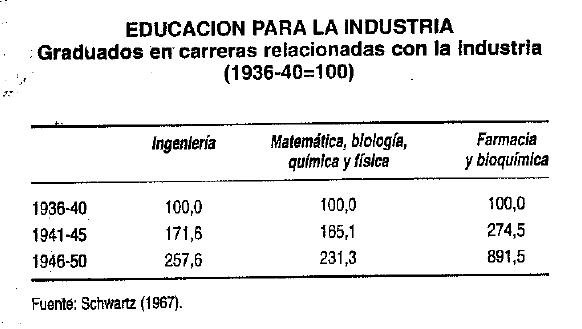
\includegraphics[scale=0.75]{uni3_politicas03}
   \label{fig:uni1_01}
\end{figure} 
  \end{frame}



    

\begin{frame}\frametitle{Desarrollo industrial (cont.)}
    \begin{itemize}\itemsep 10pt
    \item Hay muchas discrepancias entre los autores en relación al
      desempeño industrial en este período --las cifras del
      crecimiento de la actividad industrial eran entre 3.4\% y 7.5\%
      \item Algunas limitaciones evidentes $\longrightarrow$ limitada
        escala debido al pequeño mercado interno; rechazo inicial al K
        extranjero; poco énfasis en productividad
        \item En ultima instancia, esta política industrial fue
          posible gracias a los fenomenales precios de los commodities
          argentinos --transferencia intersectorial de ingresos
    \end{itemize}
      \end{frame}
  


\begin{frame}\frametitle{La marginación del sector rural}
    \begin{itemize}\itemsep 10pt
    \item Perón contó con una coyuntura externa fenomenal en sus
      primeros 3 años de gobierno $\longrightarrow$ mayores TIE del
      siglo (contraste con años 30)
      \item Así como la JNG promovía precios mínimos a los
        productores, Perón la transormó en el IAPI que monopolizó el
        comercio de cereales y oleaginosas
        \item El IAPI compraba las cosechas a agricultores y las
          vendía interna y externamente --ganancia favorable con TIE crecientes
              \end{itemize}
      \end{frame}





  \begin{frame}\frametitle{La marginación del sector rural (cont.)}
\begin{figure}[hxtbp]\vspace{0cm}
  \centering
  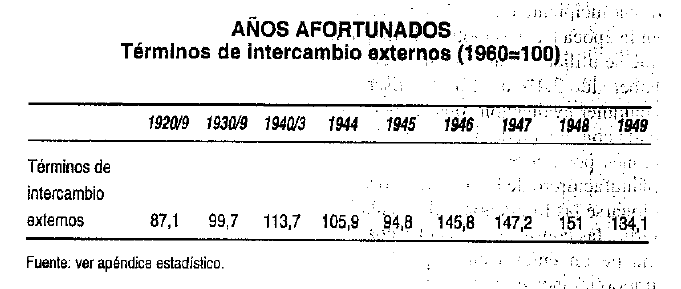
\includegraphics[scale=0.75]{uni3_politicas04}
   \label{fig:uni1_01}
\end{figure} 
  \end{frame}

      

      \begin{frame}\frametitle{La marginación del sector rural (cont.)}
    \begin{itemize}\itemsep 10pt
    \item Las ganancias del IAPI sirvieron para mantener el gasto
      público en continuo aumento. Además, sirvió para desligar los
      precios locales (de alimentos) de los internacionales
      \item Sin la intervención del IAPI, hubieran sucedido una de dos
        cosas: 1) mermado salario real (via mayores precios de
        canasta); 2) mermada rentabilidad industrial (si se pretendía
        mantener el salario real constante)
        \item Este ``triángulo redistributivo'' se asentaba en: 1)
          sector rural (dador); 2) sector urbano (receptor); 3) Estado
          (receptor). 
              \end{itemize}
      \end{frame}
  




  \begin{frame}\frametitle{La marginación del sector rural (cont.)}
\begin{figure}[hxtbp]\vspace{0cm}
  \centering
  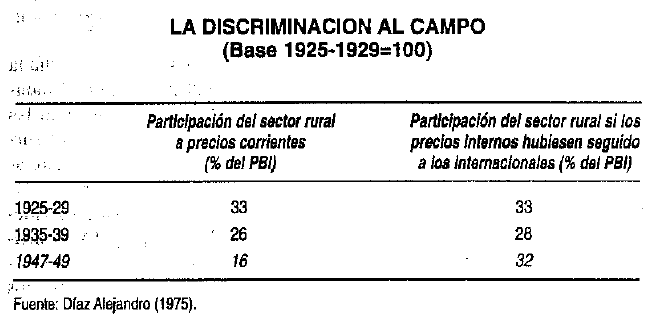
\includegraphics[scale=0.75]{uni3_politicas05}
   \label{fig:uni1_01}
\end{figure} 
  \end{frame}

      

      
      \begin{frame}\frametitle{La marginación del sector rural (cont.)}
        \begin{block}{Funcionamiento del esquema}
            El crecimiento salarial (costo a la industria) promovido
            por el gobierno era compensado por crédito barato y
            subsidiado (beneficio a la industria). El gobierno
            financiaba expansion de gasto y empleo público con el
            margen que dejaba IAPI. Esta situación dejaba entrever un
            riesgo: ante el cambio en las condiciones externas 
              \end{block}
      \end{frame}
  

        \begin{frame}\frametitle{La marginación del sector rural (cont.)}
    \begin{itemize}\itemsep 10pt
    \item Un fenómeno adicional (de equilibrio general) fue el aumento
      del costo de los productores rurales por la necesidad de
      aumentar salarios para eliminar brecha con el salario urbano
      \item También había aumentado el salario de peones a través de
        algunas disposiciones del gobierno
        \item El sistema de arrendamientos entró en crisis debido al
          congelamiento de alquileres y a la erosión de las rentas por
          la inflación
          \item En parte la gradual y sostenida caída del area
            sembrada puede explicarse por la medidas desfavorables 
              \end{itemize}
      \end{frame}
  


  \begin{frame}\frametitle{La marginación del sector rural (cont.)}
\begin{figure}[hxtbp]\vspace{0cm}
  \centering
  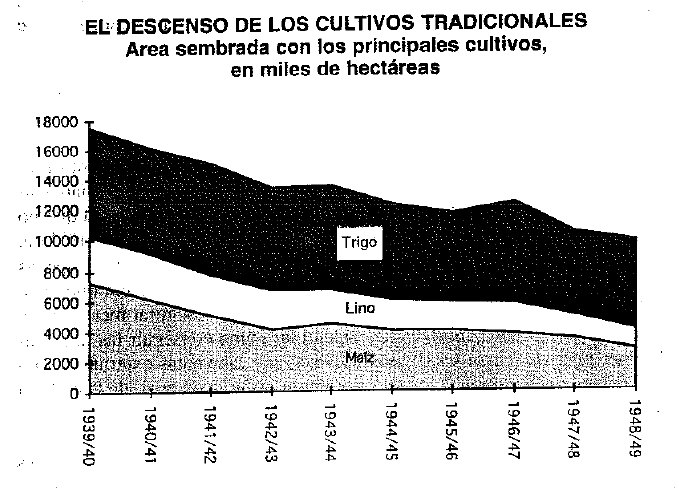
\includegraphics[scale=0.75]{uni3_politicas06}
   \label{fig:uni1_01}
\end{figure} 
  \end{frame}
      
      
                 
\end{document}

      